\documentclass{standalone}
\usepackage{tikz}
\usetikzlibrary{arrows.meta}

\begin{document}

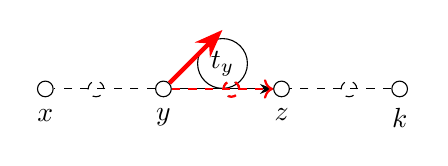
\begin{tikzpicture}[scale=1.5, every node/.style={circle, draw, inner sep=2pt, minimum size=4pt}]
    \node[label=below:$x$] (x) at (0,0) {};
    \node[label=below:$y$] (y) at (1,0) {};
    \node[label=below:$z$] (z) at (2,0) {};
    \node[label=below:$k$] (k) at (3,0) {};

    % Dotted edges of the cycle C
    \draw[dashed] (y) -- node[left] {} (x);
    \draw[dashed] (z) -- node[right] {} (y);
    \draw[dashed] (k) -- node[right] {} (z);

    % Solid edge yz with label t_y
    \draw[-Stealth] (y) -- node[pos=0.5, above] {$t_y$} (z);

    % Dotted edge from y to z (edge e)
    \draw[red, dashed, thick, ->] (y) -- node [pos=0.5, right] {} (z);

    % Red arrow for clarity
    \draw[red, ultra thick, -Stealth] (y) -- ++(0.5,0.5);
\end{tikzpicture}

\end{document}